\documentclass[10pt,twocolumn]{article}

% use the oxycomps style file
\usepackage{oxycomps}
\usepackage{multirow}
\usepackage{ragged2e}
\usepackage{blindtext}
\graphicspath{ {./images/} }
% usage: \fixme[comments describing issue]{text to be fixed}
% define \fixme as not doing anything special
\newcommand{\fixme}[2][]{#2}
% overwrite it so it shows up as red
\renewcommand{\fixme}[2][]{\textcolor{red}{#2}}
% overwrite it again so related text shows as footnotes
%\renewcommand{\fixme}[2][]{\textcolor{red}{#2\footnote{#1}}}

% read references.bib for the bibtex data
\bibliography{references}

% include metadata in the generated pdf file
\pdfinfo{
    /Title (Course Companion: An Analysis of the Need for Course Reviews at Occidental College)
    /Author (Kyla Allen)
}

% set the title and author information
\title{Course Companion: An Analysis of the Need for Course Reviews at Occidental College}
\author{Kyla Allen}
\affiliation{Occidental College}
\email{kallen2@oxy.edu}

\begin{document}

\maketitle

\section{Problem Context\footnote{\href{https://www.overleaf.com/8949248344rhtkzfvbcxjs}{Link to Overleaf Project}}}
The goal of this project is to create a web app that acts as a platform for students interested in the Computer Science major at Occidental College to rate and provide feedback on their experiences within the classes they have taken. Eventually, other students will be able to use that feedback in order to make informed decisions when putting together their class schedules.

\subsection{Introduction}
Education is a critical aspect of an individual's personal and professional development. At the heart of any academic journey is course selection, which can be a daunting task for students. With limited information on course content, workload, and professor quality, students are often left to navigate course selection based on limited information. In this section, I will explore the societal and personal importance of creating a platform where students are able to share feedback on the courses they've taken.

\subsection{Personal Importance}
Although I will not personally benefit from the website I created, as I will be a senior by the time it is completed, I find it important to contribute to my college community and provide a useful resource for current and future students. As an avid user of similar websites, I understand the value of having a platform where students can access information about courses and instructors. By creating a platform specific to Occidental College, I hope to provide a tailored experience for my peers and contribute to the improvement of our academic community.


\subsection{The Importance of User Feedback}
The emphasis on user feedback, specifically through the implementation of user testing, serves as a strategic solution for creating a helpful resource for the Occidental community. User feedback allows the project creator to understand and adhere to the needs of the community. Without user testing, creators cannot fully understand what the problem is and how to best mitigate said problem.

User testing through user-centered design is a methodical approach to evaluating the usability, functionality, and overall user experience of a project or platform \cite{mao2005}. By actively involving members of the Occidental community in the testing process, I aim to gain valuable insights into how the intended users interact with and perceive my site. This direct engagement allows for a nuanced understanding of the specific needs, preferences, and challenges faced by the community.

Understanding the needs of the Occidental community is paramount for the project's success. User feedback serves as a lens through which the creator may uncover areas for improvement and refine the project's objectives. Without this direct input from users, creators might find themselves working in isolation, potentially missing crucial nuances that are evident only through the eyes and experiences of the community members.

Moreover, user testing provides a mechanism for creators to gauge the effectiveness of their solutions to identified problems. It's not just about understanding the issues at hand, but also about validating that the implemented solutions align with the expectations and preferences of the scope. This iterative feedback loop ensures that adjustments can consistently be made in real-time, creating a dynamic and responsive development process.

Overall, the absence of user testing introduces the risk of misalignment between the project and the community it aims to serve. Without a clear understanding of how users navigate and utilize the resource, creators may inadvertently introduce features that are irrelevant or overlook functionalities that are essential to the community.

%this section is important get citations
\subsection{The Importance of Peer Feedback}
In general, college students have a very limited amount of information available to them when it comes to choosing potential classes. At Occidental College, and many other schools, course descriptions are about three to four sentences and fail to provide an accurate representation of the course's content or workload. Additionally, there is often a lack of information on professor quality, which can significantly impact a student's experience in a course. As a result, students may end up taking courses that do not align with their interests, goals, or abilities, leading to lower academic performance and overall dissatisfaction.  By prioritizing real experiences and insights from peers, students gain valuable perspectives on course content, workload, and professor quality. This approach enhances decision-making, reducing the likelihood of dissatisfaction and schedule rearrangements mid-semester.

Peer feedback can be an effective solution to the challenges that the course selection process presents. Reading comments from other students who have taken a course can provide valuable insights into the course's content, workload, and professor quality. Peer feedback can also help students better understand how a course aligns with their expectations for the class, which makes them less likely to drop and be forced to rearrange their schedule after the semester has already started.

\subsection{Impact on Student Success}
The impact of a platform for sharing course feedback can be significant on student success and satisfaction. It has been proven that available information on professor reputation and other class related information greatly influences students' course decisions \cite{brown15}. By providing students with more information on the courses they are considering, they can make more informed decisions that align with their interests, goals, and abilities. The platform can also foster increased engagement and collaboration among students, leading to a more vibrant academic community.


\section{Technical Background}
\subsection{Project Focus}
In the beginning of my project, I adjusted the initial technical plan to better match the project's priorities and goals. While the original plan outlined the utilization of both front-end and back-end technologies, the final implementation primarily focused on front-end development, specifically emphasizing user testing.

\subsection{Front-End Development}
The project's front-end was built with React, a versatile JavaScript library, known for handling complex user interfaces efficiently. TypeScript was added for improved type safety and code maintainability. Styling was done using CSS to create a polished and responsive user interface.

\subsection{Libraries and Tools}
Several libraries were used in shaping the functionality and aesthetics of the web app. These include:

\begin{itemize}
  \item \textbf{Infragistics:} Used for the creation of visually appealing and interactive pie charts, providing a dynamic representation of class feedback data.
  
  \item \textbf{Bootstrap:} Utilized for styling purposes, Bootstrap contributed to the overall design consistency and responsiveness of the web application.
  
  \item \textbf{PapaParse:} Facilitated the parsing of CSV files containing pie chart data and class review information, enhancing the efficiency of data processing within the application.
\end{itemize}

\subsection{Strategic Decision}
In the interest of project focus and efficiency, the decision was made to leave out any back-end development, and instead, concentrate efforts on refining the user interface and conducting thorough user testing. This strategic shift allowed for a more concentrated exploration of the user experience, ensuring that the front-end met user expectations and effectively served the intended purpose.

The revised technical approach aligns with the project's core objective of creating a user-friendly platform for students to share and access class-related feedback. This emphasis on the front-end and user testing reflects a pragmatic and user-centered strategy in the development and refinement of my web application.


\section{Prior Work}

Although there are a few sites similar to the website I created, no site exists that is specific to the Occidental College community. While I drew inspiration from similar sites such as RateMyProfessor.com and counts.oxy.edu, my approach presents enough distinctiveness to offer a fresh perspective in the market.

\subsection{Peer Evaluation and User-Centered Design (UCD) Practice} 
In academia, peer evaluation assesses individuals' work, a practice paralleled in the industry's adoption of UCD. UCD, emphasizing user involvement, is crucial for enhancing product usability \cite{mao2005}. Peer evaluation, alongside with UCD, is used to provide feedback, assess performance, and to help improve skills and abilities.

There are several types of peer evaluation methods, including self-evaluation, group evaluations, and instructor-led evaluations. Self-evaluation allows students to assess their own progress and to identify areas where they need to improve. Group evaluations involve evaluating the work of peers within a group setting. Instructor-led evaluations are typically used to evaluate the overall progress of a class or group of students. 

Commonly used UCD methods include iterative design, usability evaluation, task analysis, informal expert review, and field studies. \cite{mao2005}. Iterative design is a method where designers refine a product by creating prototypes, collecting user feedback, and making improvements through multiple cycles. This iterative process ensures that the design continually aligns with user needs and expectations. Usability evaluation involves assessing a system's usability by observing users interact with it. Methods such as usability testing, heuristic evaluation, and cognitive walk-throughs are employed to identify and address potential usability issues, ensuring a positive user experience. Task analysis breaks down complex tasks into smaller steps to understand how users interact with a system to achieve specific goals. By analyzing user actions and decision points, designers optimize the design for efficiency and effectiveness in task completion. In an informal expert review, usability experts evaluate an interface based on their knowledge of usability principles. This method relies on the expertise of professionals to identify potential issues and suggest improvements in alignment with usability guidelines. Field studies involve observing users in their natural environments to understand real-world interactions with a product or service. 

Throughout this project, I have done multiple rounds of user testing in the form of peer evaluation, and attempted to use many of the UCD methods listed above. For the duration of my project, I based my approach to user testing on both my feedback from my comps Professor, Justin Li, and the information provided within the following papers: "The state of user-centered design practice", "It Would Be Cool to Get Stampeded by Dinosaurs”: Analyzing Children's Conceptual Model of AR Headsets Through Co-Design", and "Glancee: An Adaptable System for Instructors to Grasp Student Learning Status in Synchronous Online Classes" \cite{woodward2022}\cite{mao2005}\cite{@ma2022}. "User-Centered Design Practice" introduced me to the concept of UCD and vastly improved my ability to conduct interviews, and conduct the iterative design process in a way that did not allow my personal biases to affect the outcome of the user testing \cite{mao2005}. The CHI papers, "It Would Be Cool to Get Stampeded by Dinosaurs”: Analyzing Children's Conceptual Model of AR Headsets Through Co-Design", and "Glancee: An Adaptable System for Instructors to Grasp Student Learning Status in Synchronous Online Classes", were key resources in shaping my paper structure and refining my user testing strategy \cite{woodward2022}\cite{@ma2022}. They provided practical insights on how to organize my document effectively for clarity. This included how to structure my user testing section, and more specifically the participants section. In addition, I modeled my results and discussion section after the sections within the CHI papers. The CHI literature offered valuable methodologies for user testing, helping me streamline the feedback collection process. By applying these insights, I was able to approach paper writing and user testing with a more pragmatic and efficient mindset, improving the overall quality of my work.  

\subsection{Reviews and Information in an Academic Setting}
Reviews and information platforms in an academic setting have become increasingly popular in recent years, especially with sites such as RateMyProfessors.com providing students with access to course evaluations and other academic information. These platforms in addition to Occidental College's course counts have the potential to provide students with valuable insights into course offerings and instructor performance.

However, there are limitations to these platforms. For example, reviews may be biased or incomplete, and may not provide a comprehensive picture of a course or instructor. Additionally, there may be concerns about the accuracy of information on these platforms, as well as the potential for misuse or abuse of review systems. To address these issues, it is important to implement measures such as verification of user identities and moderation of user-generated content.


\subsubsection{Rate My Professor}
RateMyProfessor is a widely recognized platform where students review and rate their professors based on teaching difficulty and overall experience. Although popular, it has faced criticism for its informal and unfiltered nature, lacking validation. The proposed course feedback system distinguishes itself by targeting Occidental College students exclusively. Focused on the course in tandem with the professor, rather than just the professor alone, this approach aims to foster a more intimate platform, mitigating concerns related to accusatory language and maintaining relevance for the specific student community. This difference avoids one of the main judgements of RateMyProfessor in that it is an unfiltered informal site that lacks validity \cite{gregory12}. By making a system that focuses partly on the course itself, the goal is to take some of the focus away from the professor and avoid accusatory or hateful language.

%reviews and information in an academic setting (rate my professor and course counts)
\subsubsection{Course Counts}
Occidental College's course counts is another tool similar to Course Companion. Course counts offers a list of all of the courses offered at Oxy within a specific semester, and gives a summary for each course listed, in addition to the professor teaching the course and the days/time block during which the course is being offered. While my website would involve the data on the course counts site, the potential feedback given on my website would go beyond the three sentence description that course counts provides for its users.

\subsubsection{Connecting Literature to the Project}
The discussed literature highlights the importance of peer evaluation in academia and the increasing popularity of platforms like RateMyProfessors.com and course counts. The proposed project seeks to leverage these concepts, offering a targeted course feedback system for Occidental College students. By focusing on the course itself and encouraging student reviews, the system aims to provide a nuanced perspective, addressing the limitations of existing platforms and enhancing the decision-making process for students when selecting courses. The distinctions in target audience and focus differentiate the proposed system, aiming to create a valuable and tailored resource for the Occidental College community.
%This section describes previous attempts at solving similar problems. This could be existing research literature, or it could be other products/apps/games that have been published. The goal is to help the reader understand what has been done and how your proposed project relates to that body of work.


\section{Methods}

\subsection{Learning the Fundamentals}
In the initial phase of my project, I focused on acquiring proficiency in React and TypeScript through online resources, particularly YouTube tutorials. I delved into tutorials provided by various creators. These tutorials played a crucial role in equipping me with the necessary skills to develop my platform.

The major focus of my project involved extensive user testing, with a primary emphasis on the interview process and subsequent contextual inquiries through iterative design \cite{mao2005}.

\subsection{User Testing and Interview Approach}
In conducting interviews and user testing for my project, I embraced the principles of User-Centered Design (UCD) through an iterative process and contextual inquiry. Following a UCD approach, the focus was on understanding and addressing the needs of users to enhance the overall user experience.


\subsection{Participants}
The participants in the interviews and the user testing sessions were all potentially intended Computer Science majors or already majoring in Computer Science, and their ages ranged from 18-22. Some participants participated in both the interviews and multiple stages of the user testing process. 

\begin{table*}[t]  % Use [t] to place the table at the top of the page
  \centering
  \begin{tabular}{ |p{3cm}||p{3cm}|p{3cm}|p{3cm}|  }
    \hline
    \multicolumn{4}{|c|}{Participant} \\
    \hline
    Pseudonym & Age & Undeclared or CS Major & Gender\\
    \hline
    Jack   &   18  & Undeclared & M\\
    Natalie & 18  & Undeclared & F\\
    Kate & 19 & Undeclared & F\\
    Martin & 19 & Undeclared & M\\
    Amy & 22  & CS Major & F\\
    Nina & 22  & CS Major & F\\
    Mary & 22  & CS Major & F\\
    Caulder & 22  & CS Major & M\\
    \hline
  \end{tabular}
  \caption{Participants Used in Interviews \& User Testing.}
  \label{tab:participant_table}
\end{table*}

\subsection{Interviews}

To understand the user perspective and preferences in class selection, the first thing that I did on the user experience side was conduct interviews with a set of questions tailored specifically to understand the course sign up process. Participants were asked to walk through their process for signing up for classes, discussing structural considerations, timing preferences, and the role of professor/class reviews in their decision-making. Some of the questions included:
\begin{enumerate}
\item Walk me through your process for signing up for classes.
\item How often do you look at reviews of a professor/class when deciding on a class?
\item What specific things do you look for when deciding on a class?
\end{enumerate}

\subsection{Breakdown of Interview Process}

During my interviews, I tried to create a casual, conversational environment so that interviewees felt comfortable sharing as much as possible. I started by getting to know the interviewee, asking them about their grade, major, hobbies, etc.... Additionally, I often encouraged interviewees to share more details or elaborate on their points. This approach aimed to gather in-depth responses with as much detail as possible.

I avoided asking questions with just a yes or no answer. Instead, I used open-ended questions to let participants share their experiences in their own words. This way, I got more genuine and detailed responses.

Overall, each interview lasted about 15 minutes, and allowed me to start the development process with a clearer vision of what users wanted from my project.


\subsubsection{Results and Implications}

The interviews led to insightful results. For instance, participants considered timing, class structure, and professor reviews in their decision-making process. In addition, the importance of these factors evolved over time and with the progression of the major. The findings lead to considerations for the development of an Oxy-specific feedback site, including features like student-written course descriptions and strategies to encourage students to rate and review their classes.

%One student explained that, the further he gets into his major, the less he uses sites like ratemyprofessor. This is due to the options for classes become more limited as you are required to take certain classes for your major. In addition, the interviewee explained, the further one gets into their major, the more aware they are of the reputation of certain classes and professors, so the need for ratemyprofessor becomes obsolete.

The biggest result of the interview stage was the realization that students value both the professors and the classes they teach. This realization sparked a fundamental shift in my project approach, steering it away from an initial emphasis solely on class-centered reviews and identifying a need for reviews that revolved around both class and professor. 

From the interviews, I gathered that students recognize how integral professors are to the academic experience, understanding that the quality of education is reliant on both the course content and the quality of the professor delivering it. This realization prompts students to prefer both class and professor feedback, as opposed to just one or the other, encompassing not only the course structure and workload but also the professor's teaching style, how approachable they are, and their overall effectiveness in delivering the content of the class. By adapting my project to accommodate both professors and their classes, I aim to provide a more well-rounded and nuanced platform that resonates with the needs of the students in order to help guide them through the decision process for choosing classes within the Occidental Computer Science major.


\subsection{User Testing}

In the post-interview phase, I begun user testing. The implementation of drawn reviews marked the beginning of my comprehensive user-centered design (UCD) approach, particularly emphasizing iterative design and contextual inquiry. The iterative design process unfolded throughout multiple cycles, each new iteration informed by user feedback obtained within the previous cycles, while contextual inquiry influenced how I conducted myself during the participant sessions.

Contextual inquiry was used in order to dive deeper into the user experience. This method involved observing users in their natural environment while they interacted with the drawn reviews feature. By understanding the context of use, including challenges and preferences, I gained valuable insights into how users used my site to help aid their class choosing process. This process was carried out by allowing participants to walk through the drafted site (whether it be drawn out or online), while I watched how they maneuvered throughout the site and which aspects of the site they interacted with most/least.

User testing played a pivotal role in evaluating the effectiveness and user-friendliness of the reviews \cite{mao2005}. I conducted the user testing in multiple rounds through tests which involved engaging users in interactive sessions to perform specific tasks and gathering real-time feedback on their experiences. This iterative user testing process allowed for the identification of usability challenges and areas for improvement, which were then analyzed and addressed in subsequent design iterations. 

Future iterations could explore further enhancements, potentially incorporating a wider variety of UCD methodologies to continually enhance the user experience.


\begin{center} \textbf{User Testing with Hand-Drawn Reviews}\\ \end{center}


Below is the first mock-up review I used for user testing. I also used more paper to create the outer layers of the site, however this review holds the most relevance:\\


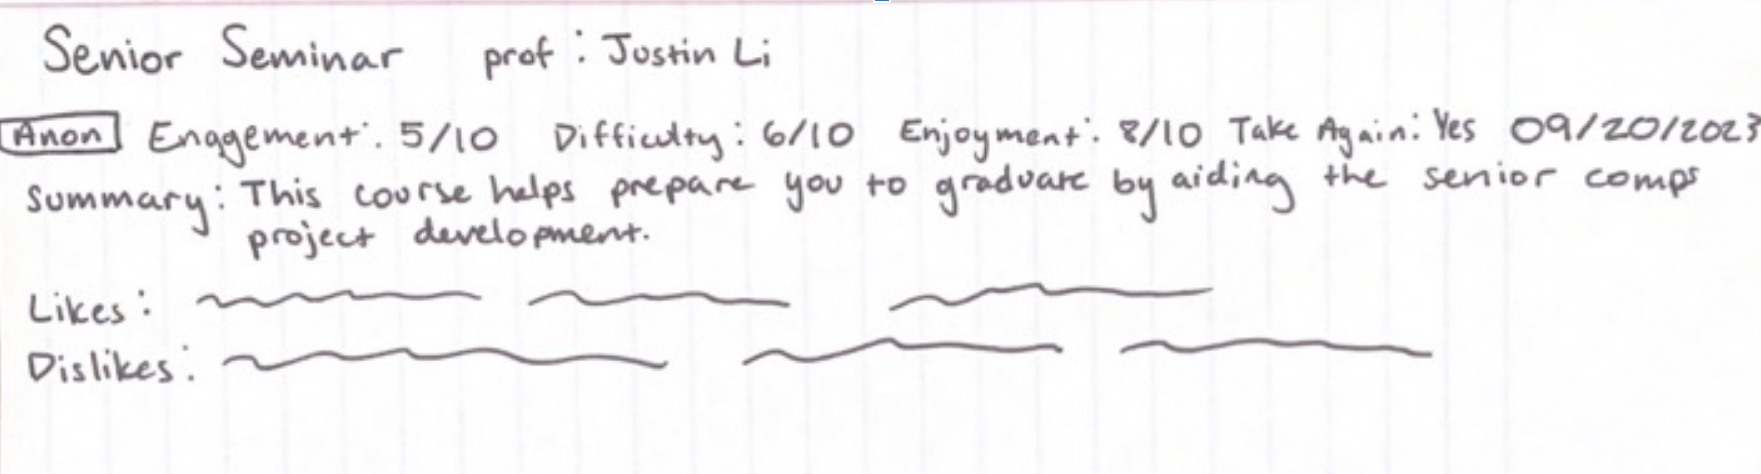
\includegraphics[scale=.25]{UT1}\\ \textbf{\footnotesize{Figure 1. 1st Version of User Tested Hand-Drawn Review}}\\

Some of the feedback I received after implementing the UCD tactics were that users needed more visual data to draw them towards the review. The participants liked the break up of the text into "Likes" and "Dislikes" as it separated a block of text into defined sections. In addition, some of the participants commented that the summary section was not useful, as they can just find that information on course counts, which every Occidental student uses. 

After receiving the feedback given through the first round of user testing, I made many changes to my hand-drawn review. First, I brainstormed ways to add more visual components to my review. I looked at ratemyprofessor and other review sites to inform my decision to ultimately create pie charts that visually represented the grade make-up and teaching style of the professor attached to the review. In addition, I took out the summary section as I felt it was not relevant to the goal of my app. I also added an interactive feature where the user can check whether they like or dislike the specific review. I added this as a way for users to give feedback to the reviewers, and to other users, in order to identify which parts of the review users found helpful/agreed with, and which parts they found unhelpful/disagreed with. Below is the second hand-drawn review for which I conducted user testing.

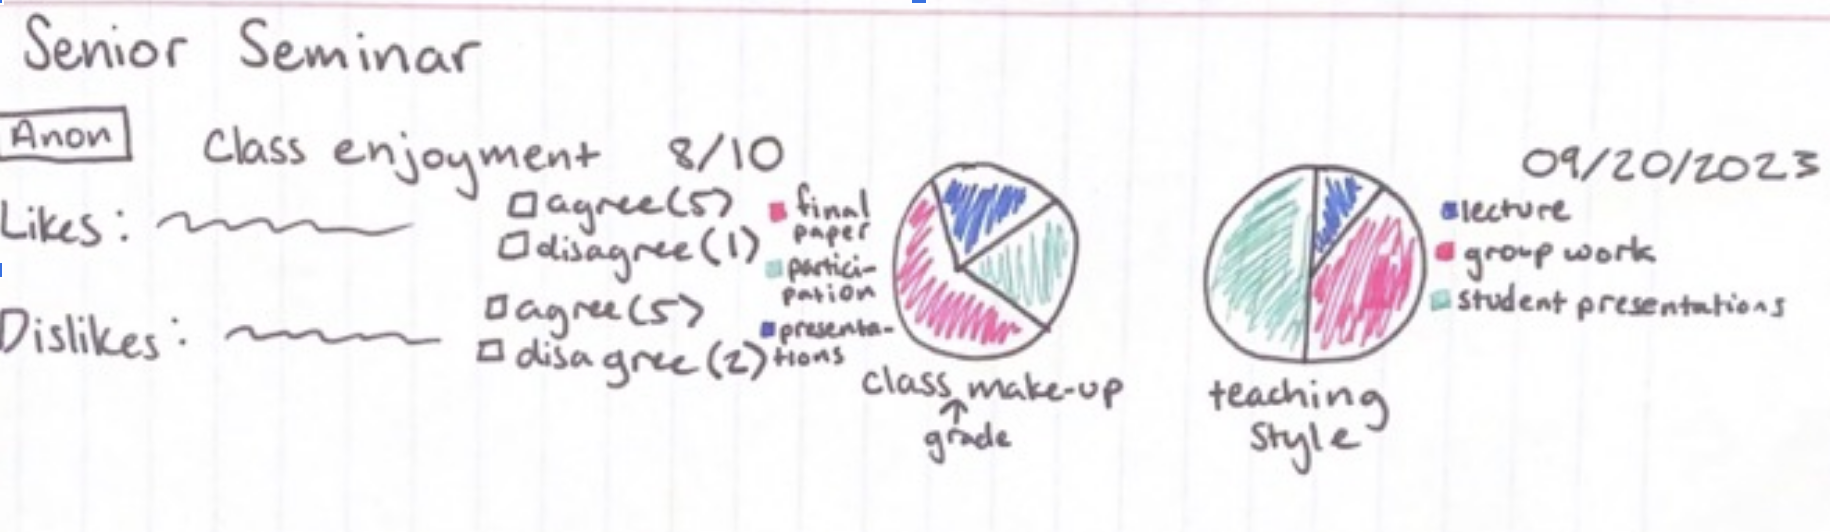
\includegraphics[scale=.25]{UT2}\\ \textbf{\footnotesize{Figure 2. 2nd Version of User Tested Hand-Drawn Review}}

Through the user testing conducted with the review above, I gathered that users engaged well with the pie charts and appreciated the way the data was structured. This is because the pie charts allowed users to see a visual synopsis of the data which allowed for a balance between reading information and interpreting graphs. Usually, in these types of reviews, it is important to have a balance between visual data and written data. In addition, I learned that users prefer more ratings at the top (i.e. difficulty out of 10, would you take again, etc...). Based on user feedback during testing, having multiple summary ratings at the top was seen as a more straightforward way to understand how the reviewer felt about the class. It eliminated the need for users to analyze the entire review to gauge the overall sentiment of the reviewer. Lastly, it was pointed out to me that I omitted the name of the professor in the review, which led to confusion amongst those who went through this round of user testing, however it should be noted that this was a personal error and should not reflect a purposeful change. Additional user feedback regarding this version will be mentioned in the sections below.\\


{\centering \textbf{User Testing with Reviews Made with Google Slides} \par}\\


After setting up the basic structure of my site, I created online mock-ups for the reviews. This allowed me to start creating fabricated reviews on the front-end of my sight. Below is an image of a section of the first version of the review I created using google slides. 

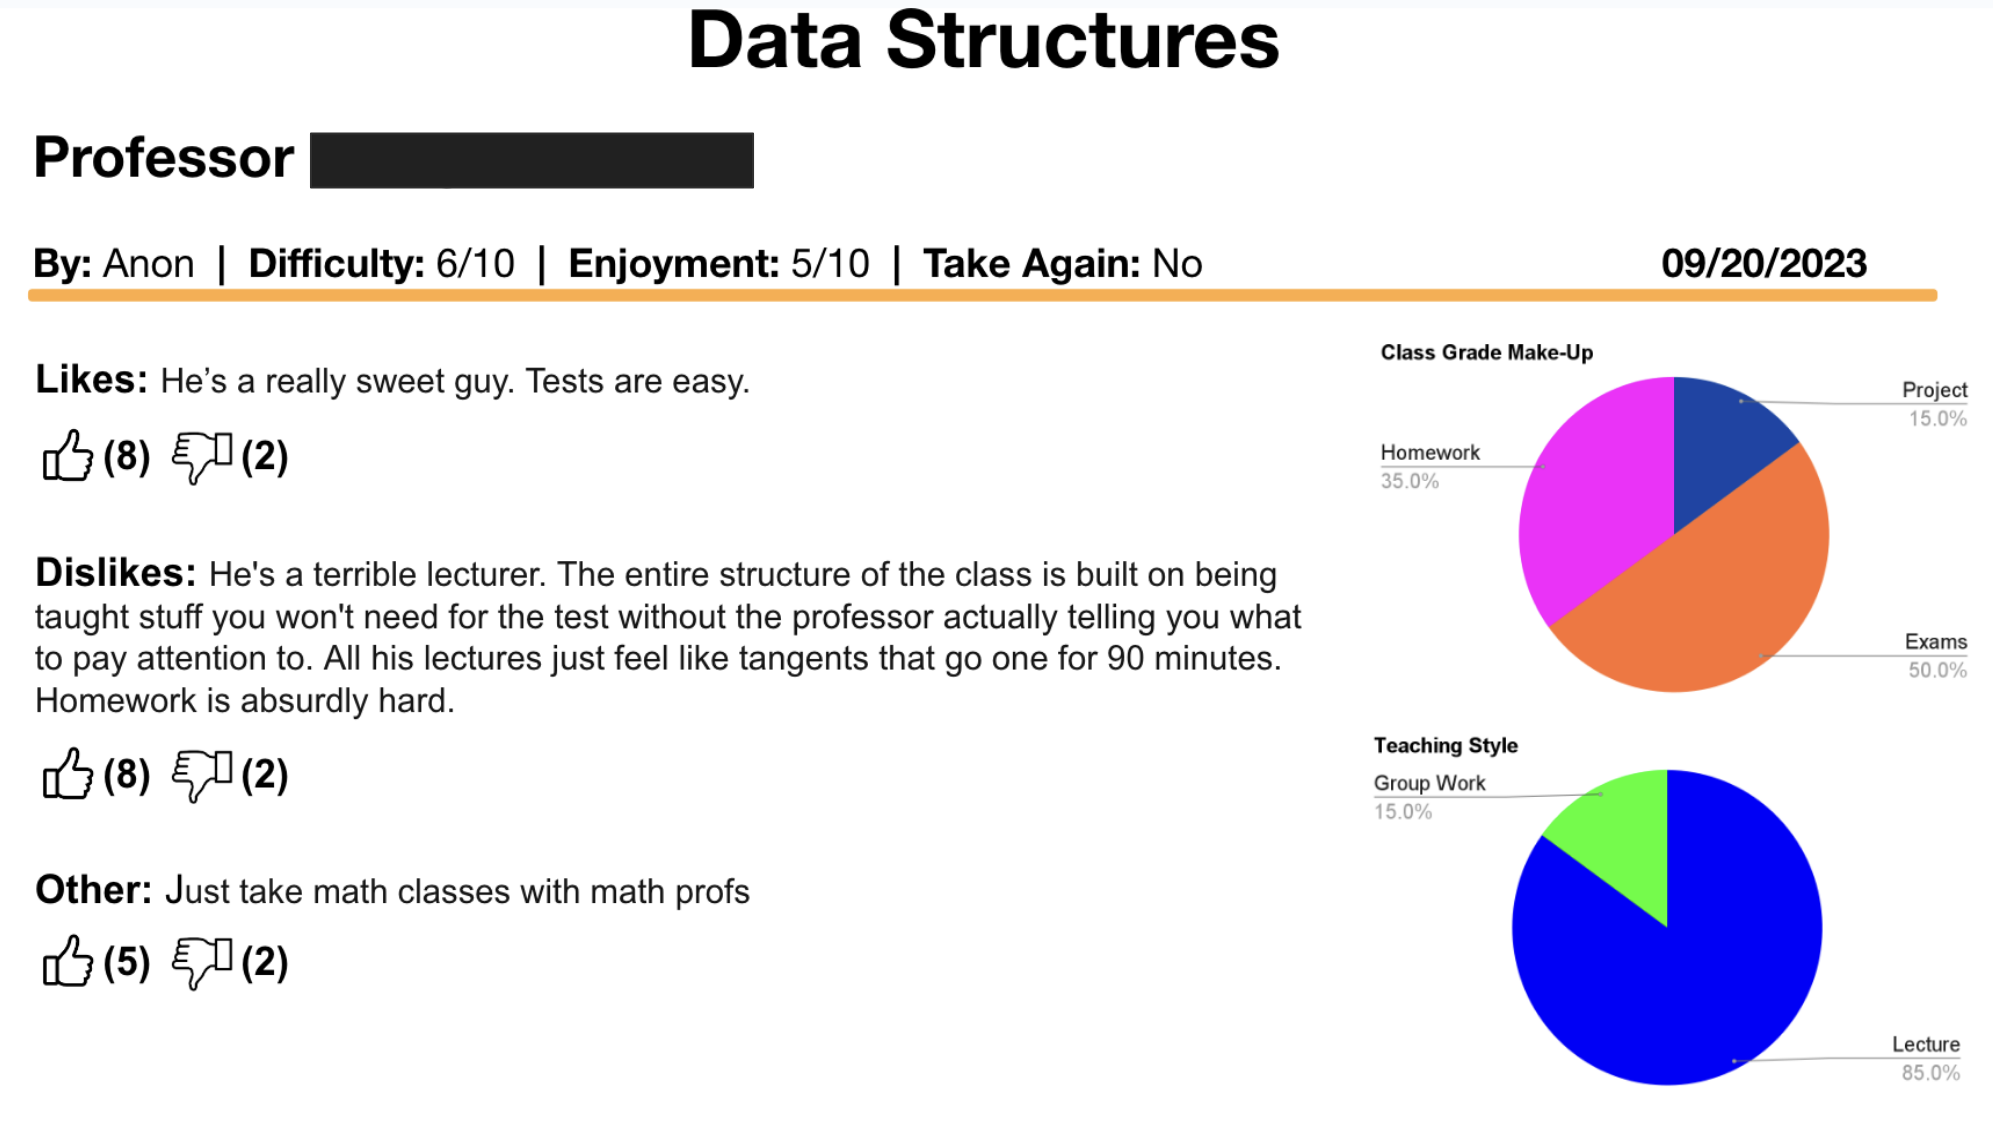
\includegraphics[scale=.25]{UT3}\\ \textbf{\footnotesize{Figure 3. 3rd Version of User Tested Review Made on Google Slides}}\\

In this review, I have included a like or dislike button in the form of a thumbs up/thumbs down which was suggested in user testing, as the dislike/like checkbox made the sections feel crowded. Participants still felt like it was important to give the option for users to provide feedback, however some felt it could be done in a more succinct manner. I felt that the appearance of a picture versus a checkbox with a description would be more user friendly and take up less space. Additionally, each section has its own set of pie charts for each professor. These pie charts were modeled after the pie charts in Figure 2.

Much of the feedback I received during this round of user testing revolved around the pie charts. While people liked the content of the pie charts and were drawn to the way it was represented, users seemed confused by the repetitiveness of the pie charts as you scroll down and see multiple reviews by the same professor. 

In addition, there was confusion regarding the thumbs up/thumbs down buttons, as they can come from anyone, so whether it was an individual agreeing with the review or thinking the review was helpful was unclear. Ultimately, I decided to limit the thumbs up/thumbs down to once at the bottom of each review, and left it up to the user to decide what the amount of likes/dislikes means to them.

By restricting the voting to a single instance, the project aims to provide more accurate and meaningful signals to users about the perceived quality or usefulness of a review. This approach helps users make informed decisions by considering a unified assessment of the community's feedback, avoiding potential confusion from scattered and unclear reactions.

Moreover, by leaving the interpretation of the number of likes or dislikes up to the individual user, the project embraces user-centered design \cite{mao2005}. Users can ascribe their own meaning to the reactions, whether viewing it as a measure of agreement, helpfulness, or overall sentiment. This flexibility acknowledges the diverse ways in which users might engage with the site, ensuring that the platform accommodates a range of user perspectives and preferences. In the future, there could be more user testing to see if there are any other types of viewer feedback that could be more helpful to students. 

Participants in user testing also inquired about classes being taken for the major or not. The reasoning being that reviews rating a high level of difficulty might hold less weight coming from a non-major. Ultimately, I decided to include this in my final round of user testing. 

I decided to include the option for users to provide their name in the "By: (Author)" section, even though it's often left as anonymous. This decision was driven by the intention to discourage the use of negative language and personal attacks in reviews. By offering the opportunity for users to take accountability for their reviews, I aimed to foster a more constructive and respectful environment \cite{ellis1984}. While it's acknowledged that anonymity can still be maintained, future considerations might involve additional user testing to explore alternative methods of balancing accountability with the freedom to express opinions openly .\\


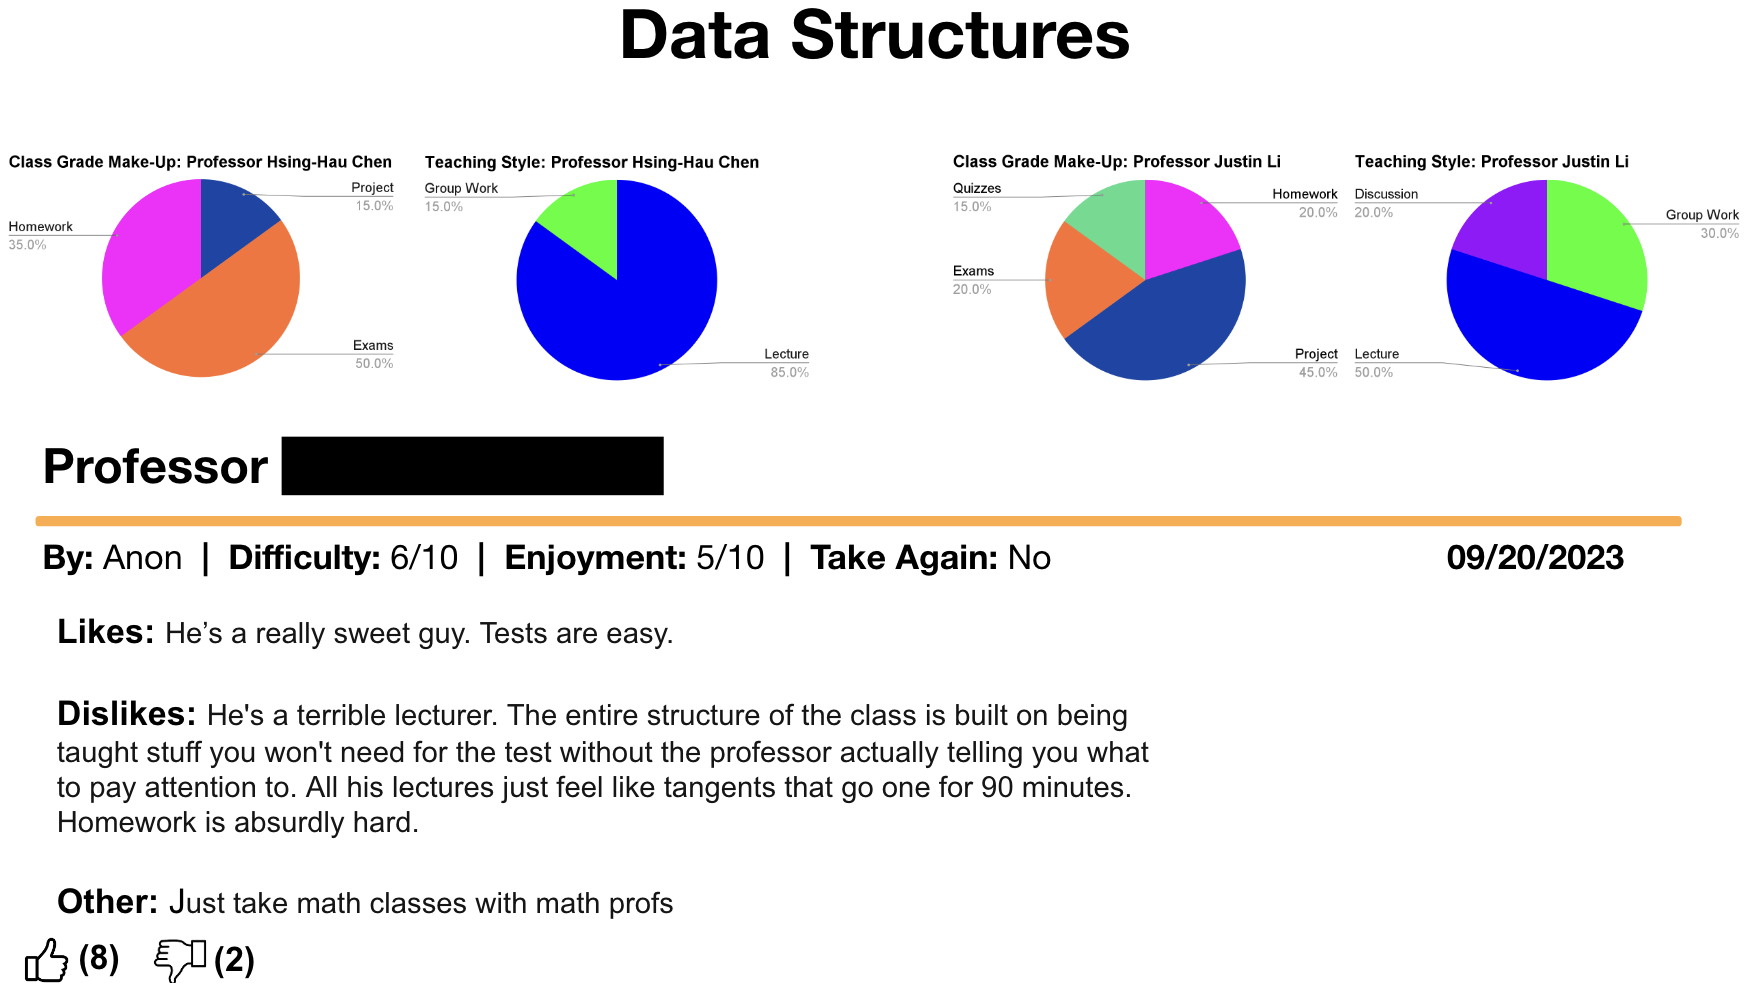
\includegraphics[scale=.27]{UT4}\\ \textbf{\footnotesize{Figure 4. 4th Version of User Tested Review Made on Google Slides}}

In this updated review, I moved the pie charts to the top of the page. This way, if students happen to be looking for a specific professor, they can see at the top all of the different professors within the review. In addition, this solution resolves the issue of the pie charts being repeated when their are multiple reviews for one professor. In order to create one set of pie charts for each professor, I can take the averages (minus any outliers) from each review and/or the average of the top (most liked) ~3 reviews. As of now, the pie charts are created using fake data, so they do not represent the real teaching styles and grade make-ups for the professors. \\


{\centering \textbf{User Testing Stage 3--Actual Website}\par}\\


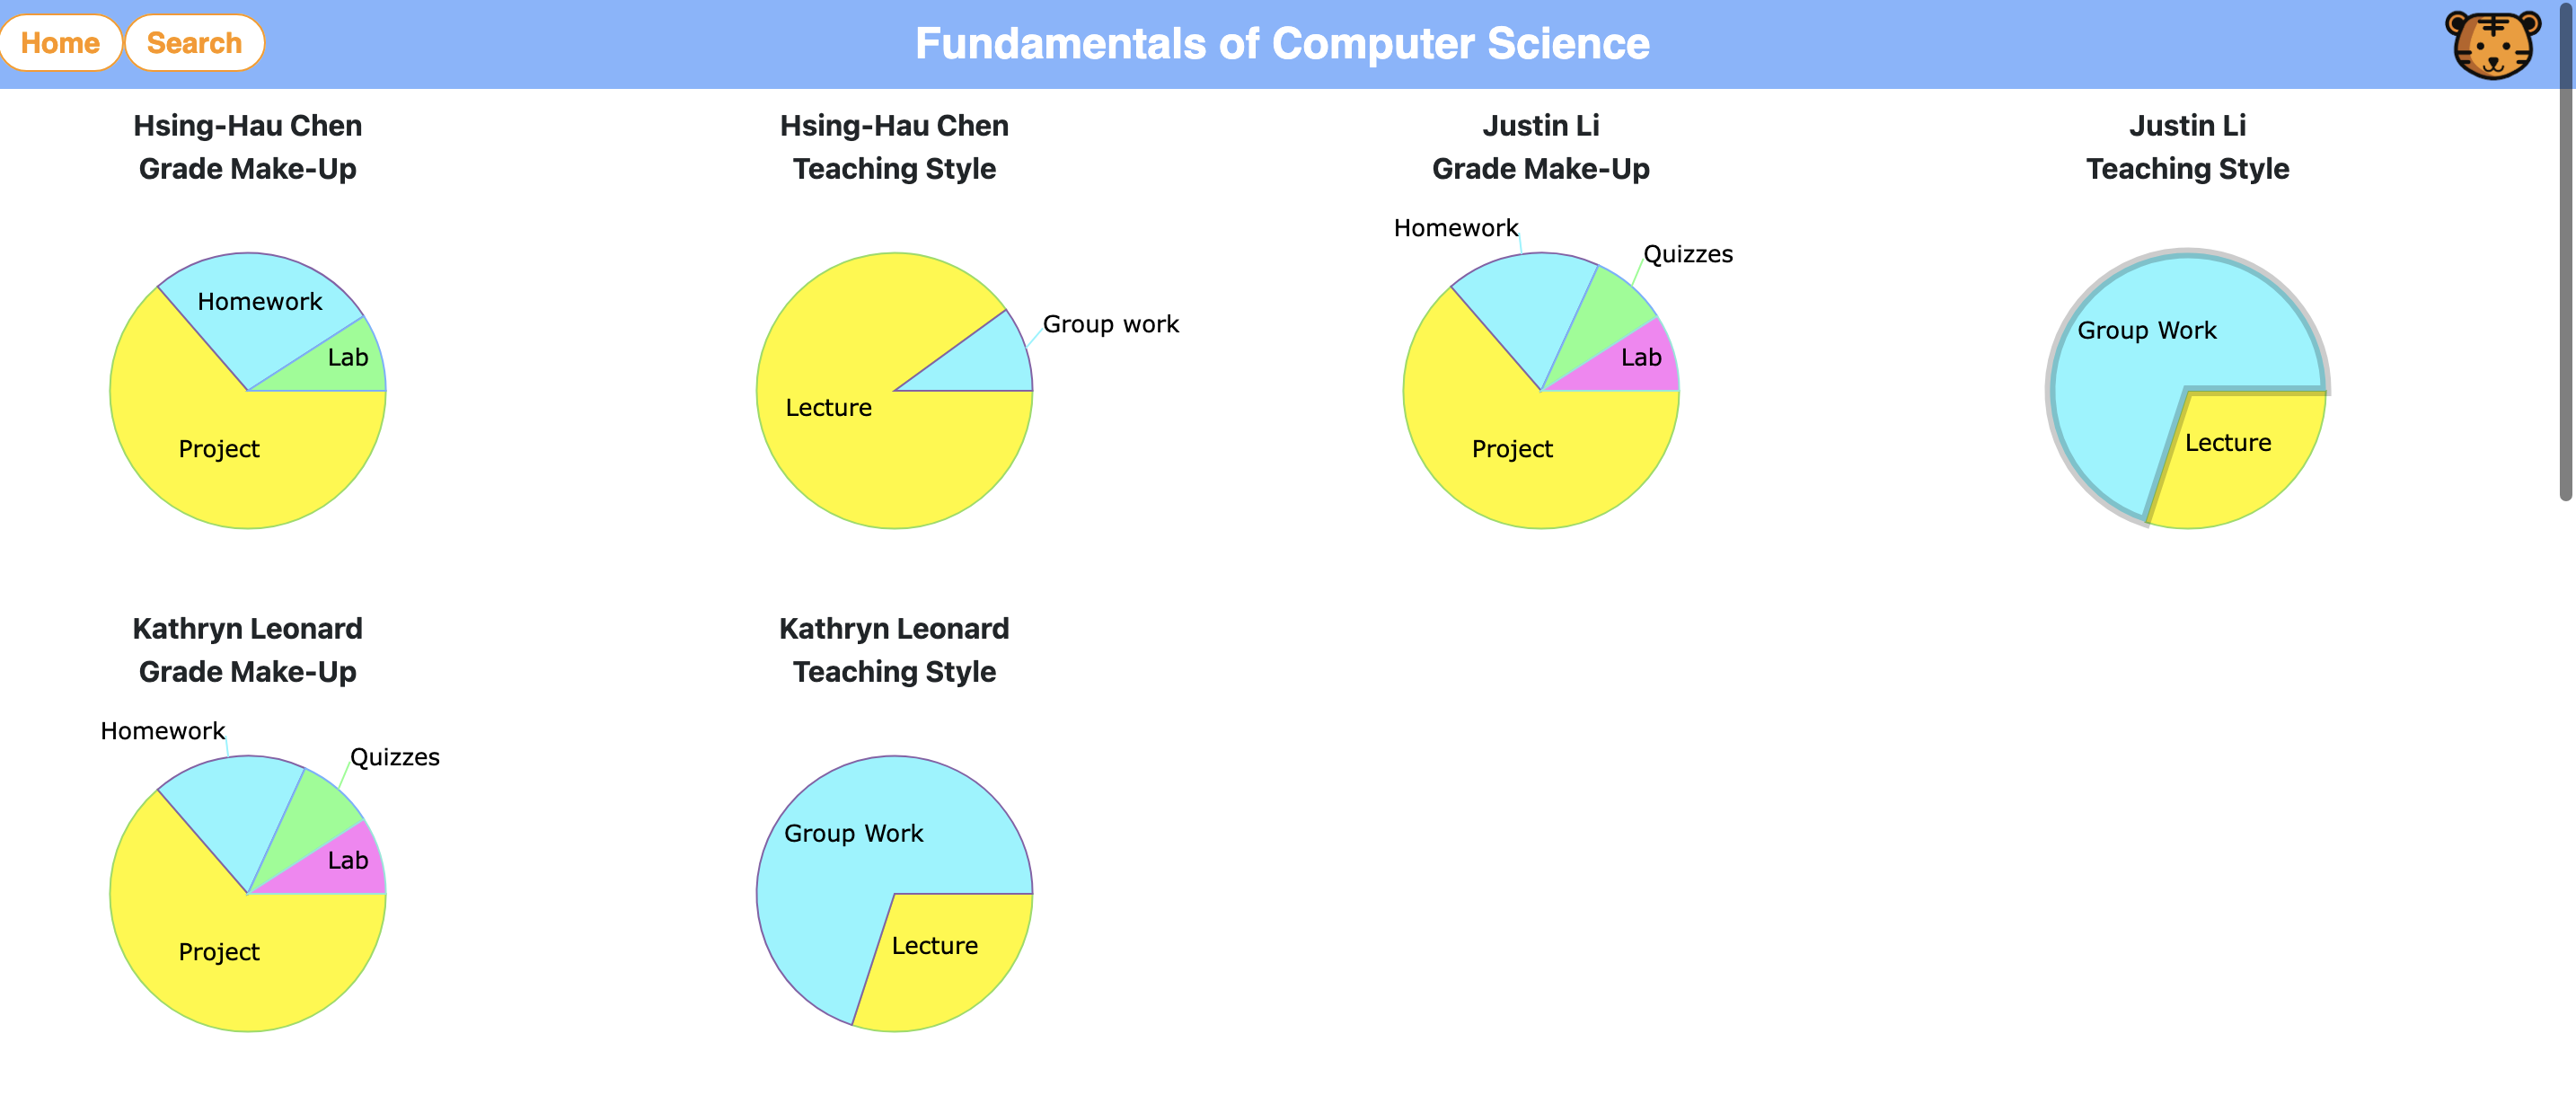
\includegraphics[scale=.165]{UT5}\\ \textbf{\footnotesize{Figure 5. Pie Charts with S}}\\


In the image above, participants in my user testing were confused regarding the repeated name of the professor within grading style. Ideally, I would put the professor's name centered in between the two pie charts, however, given the fact that the pie charts are all their own element, I struggled to figure out the label given the time constraints of the project. In the future, I hope to solve this issue in order to create more clarity and decrease repetition \cite{noname08}. \\



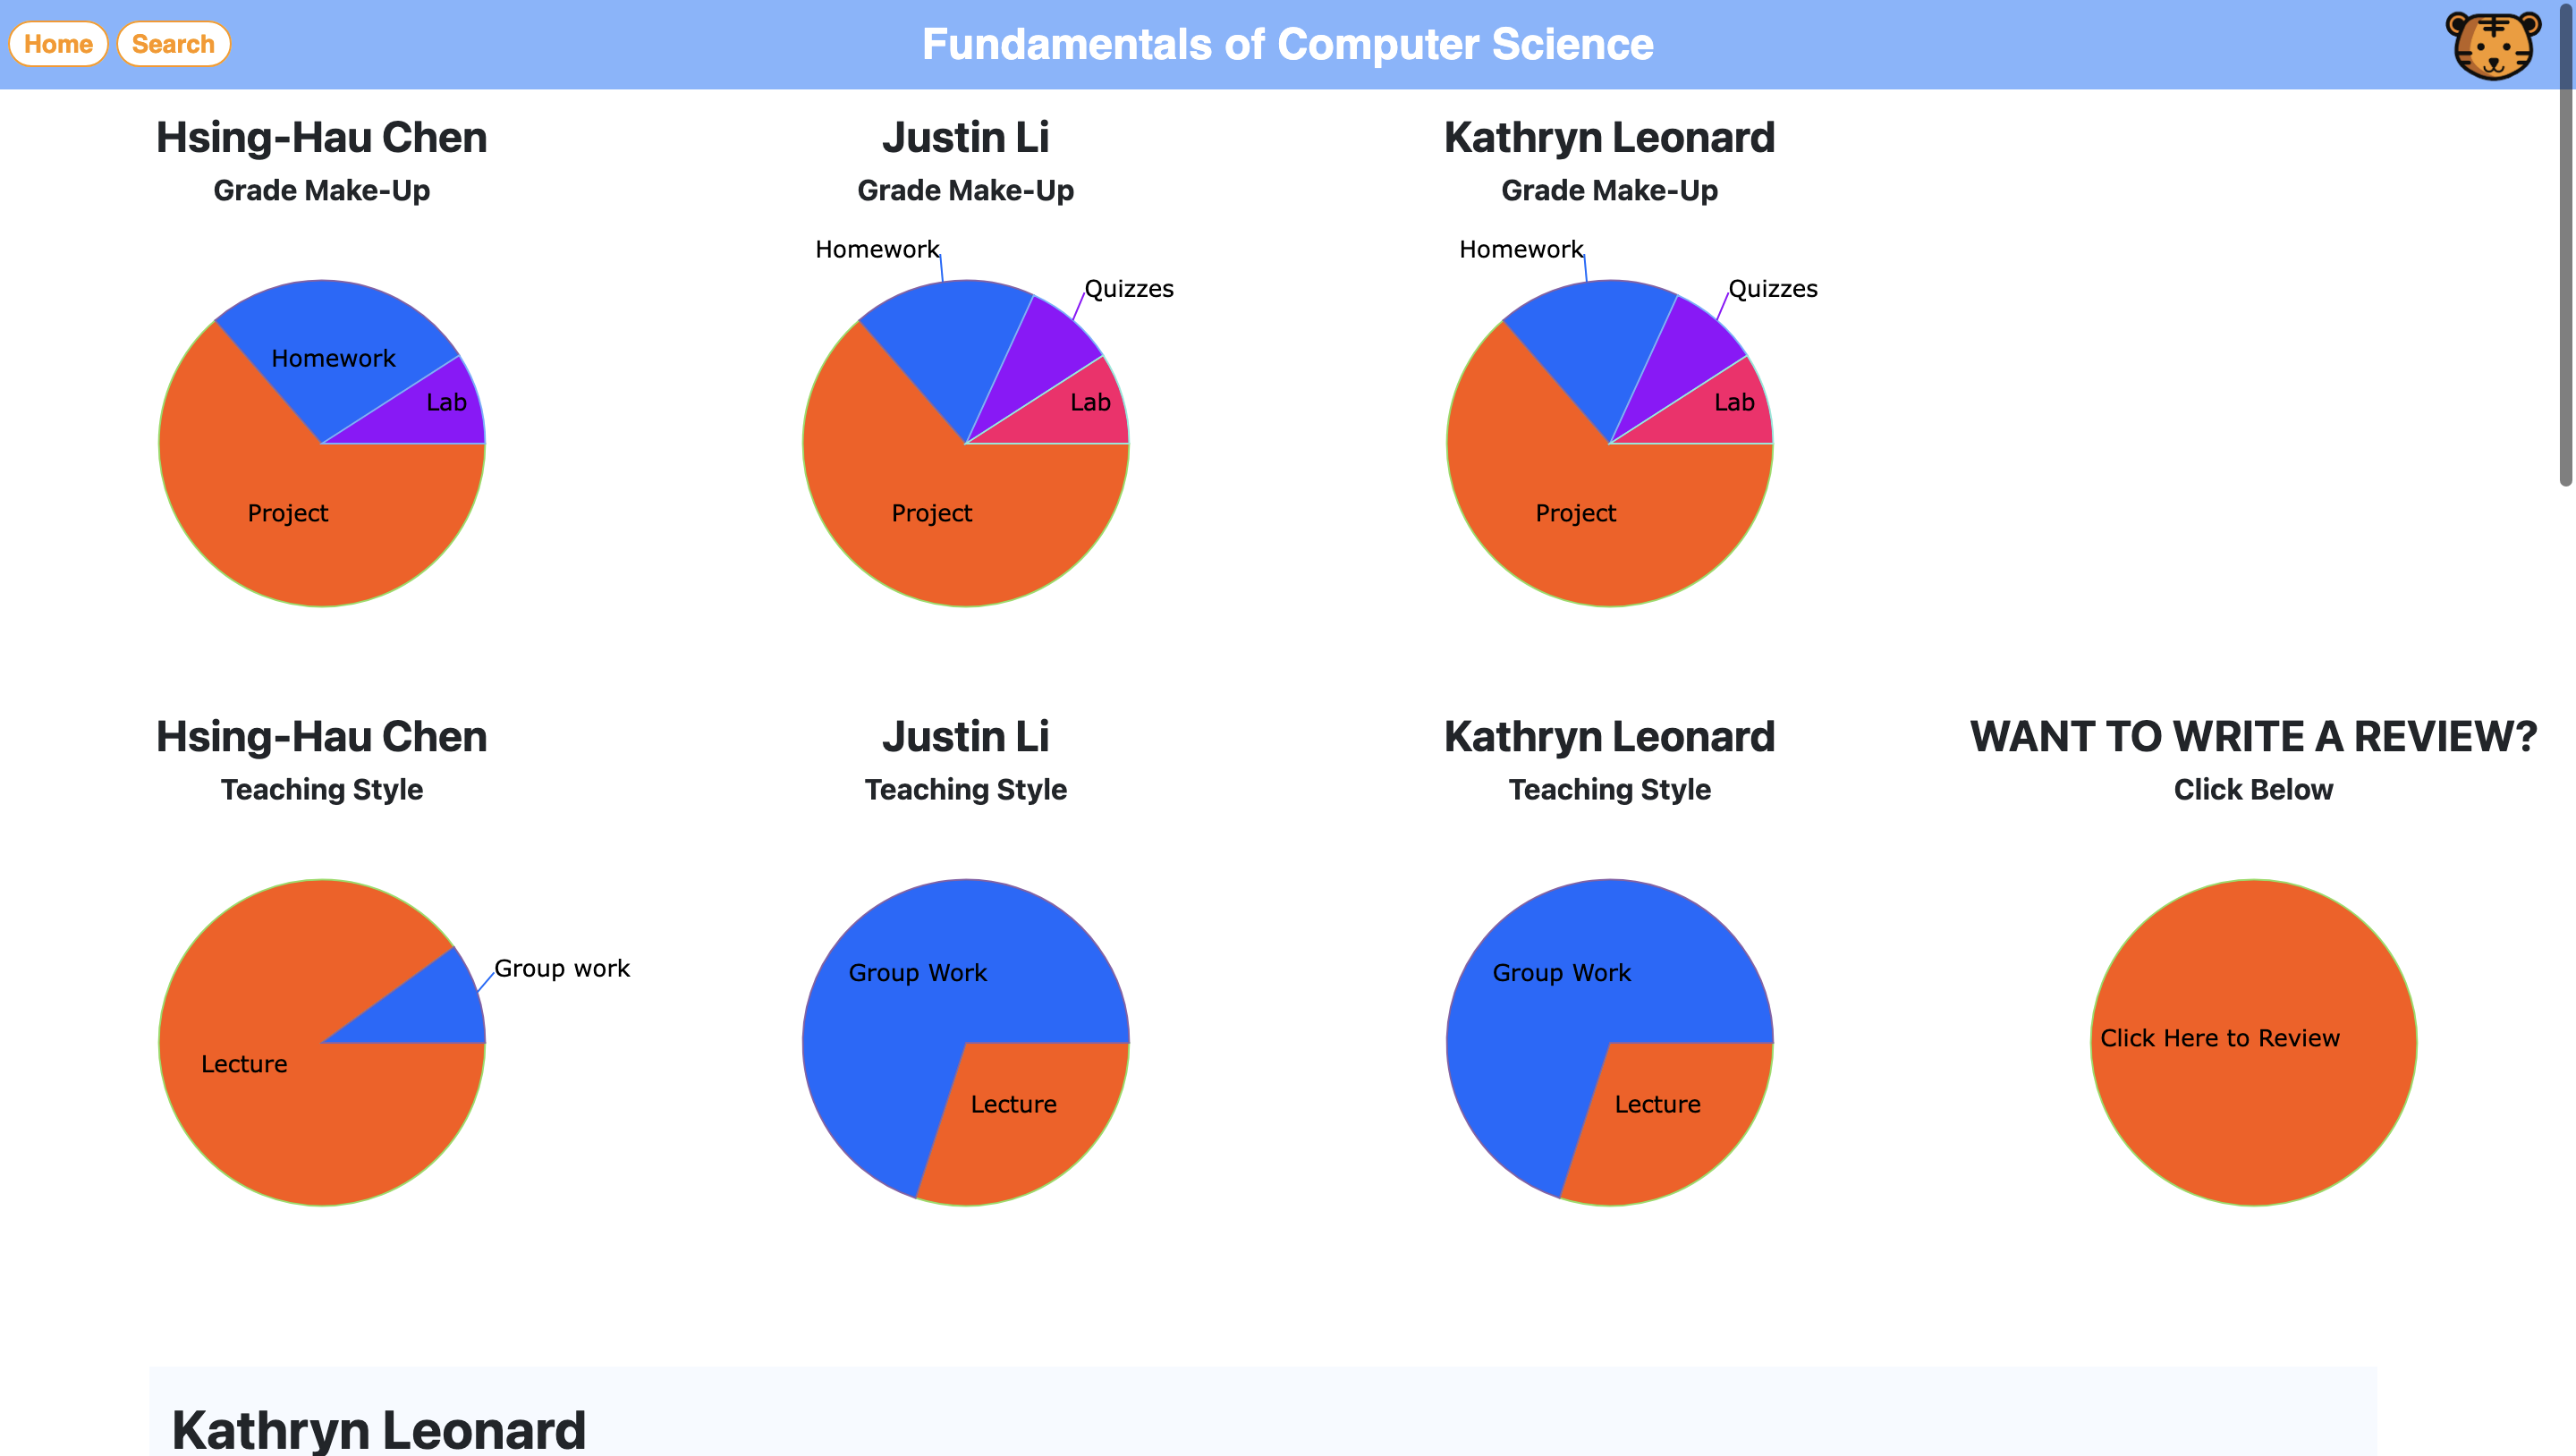
\includegraphics[scale=.15]{UT6}\\
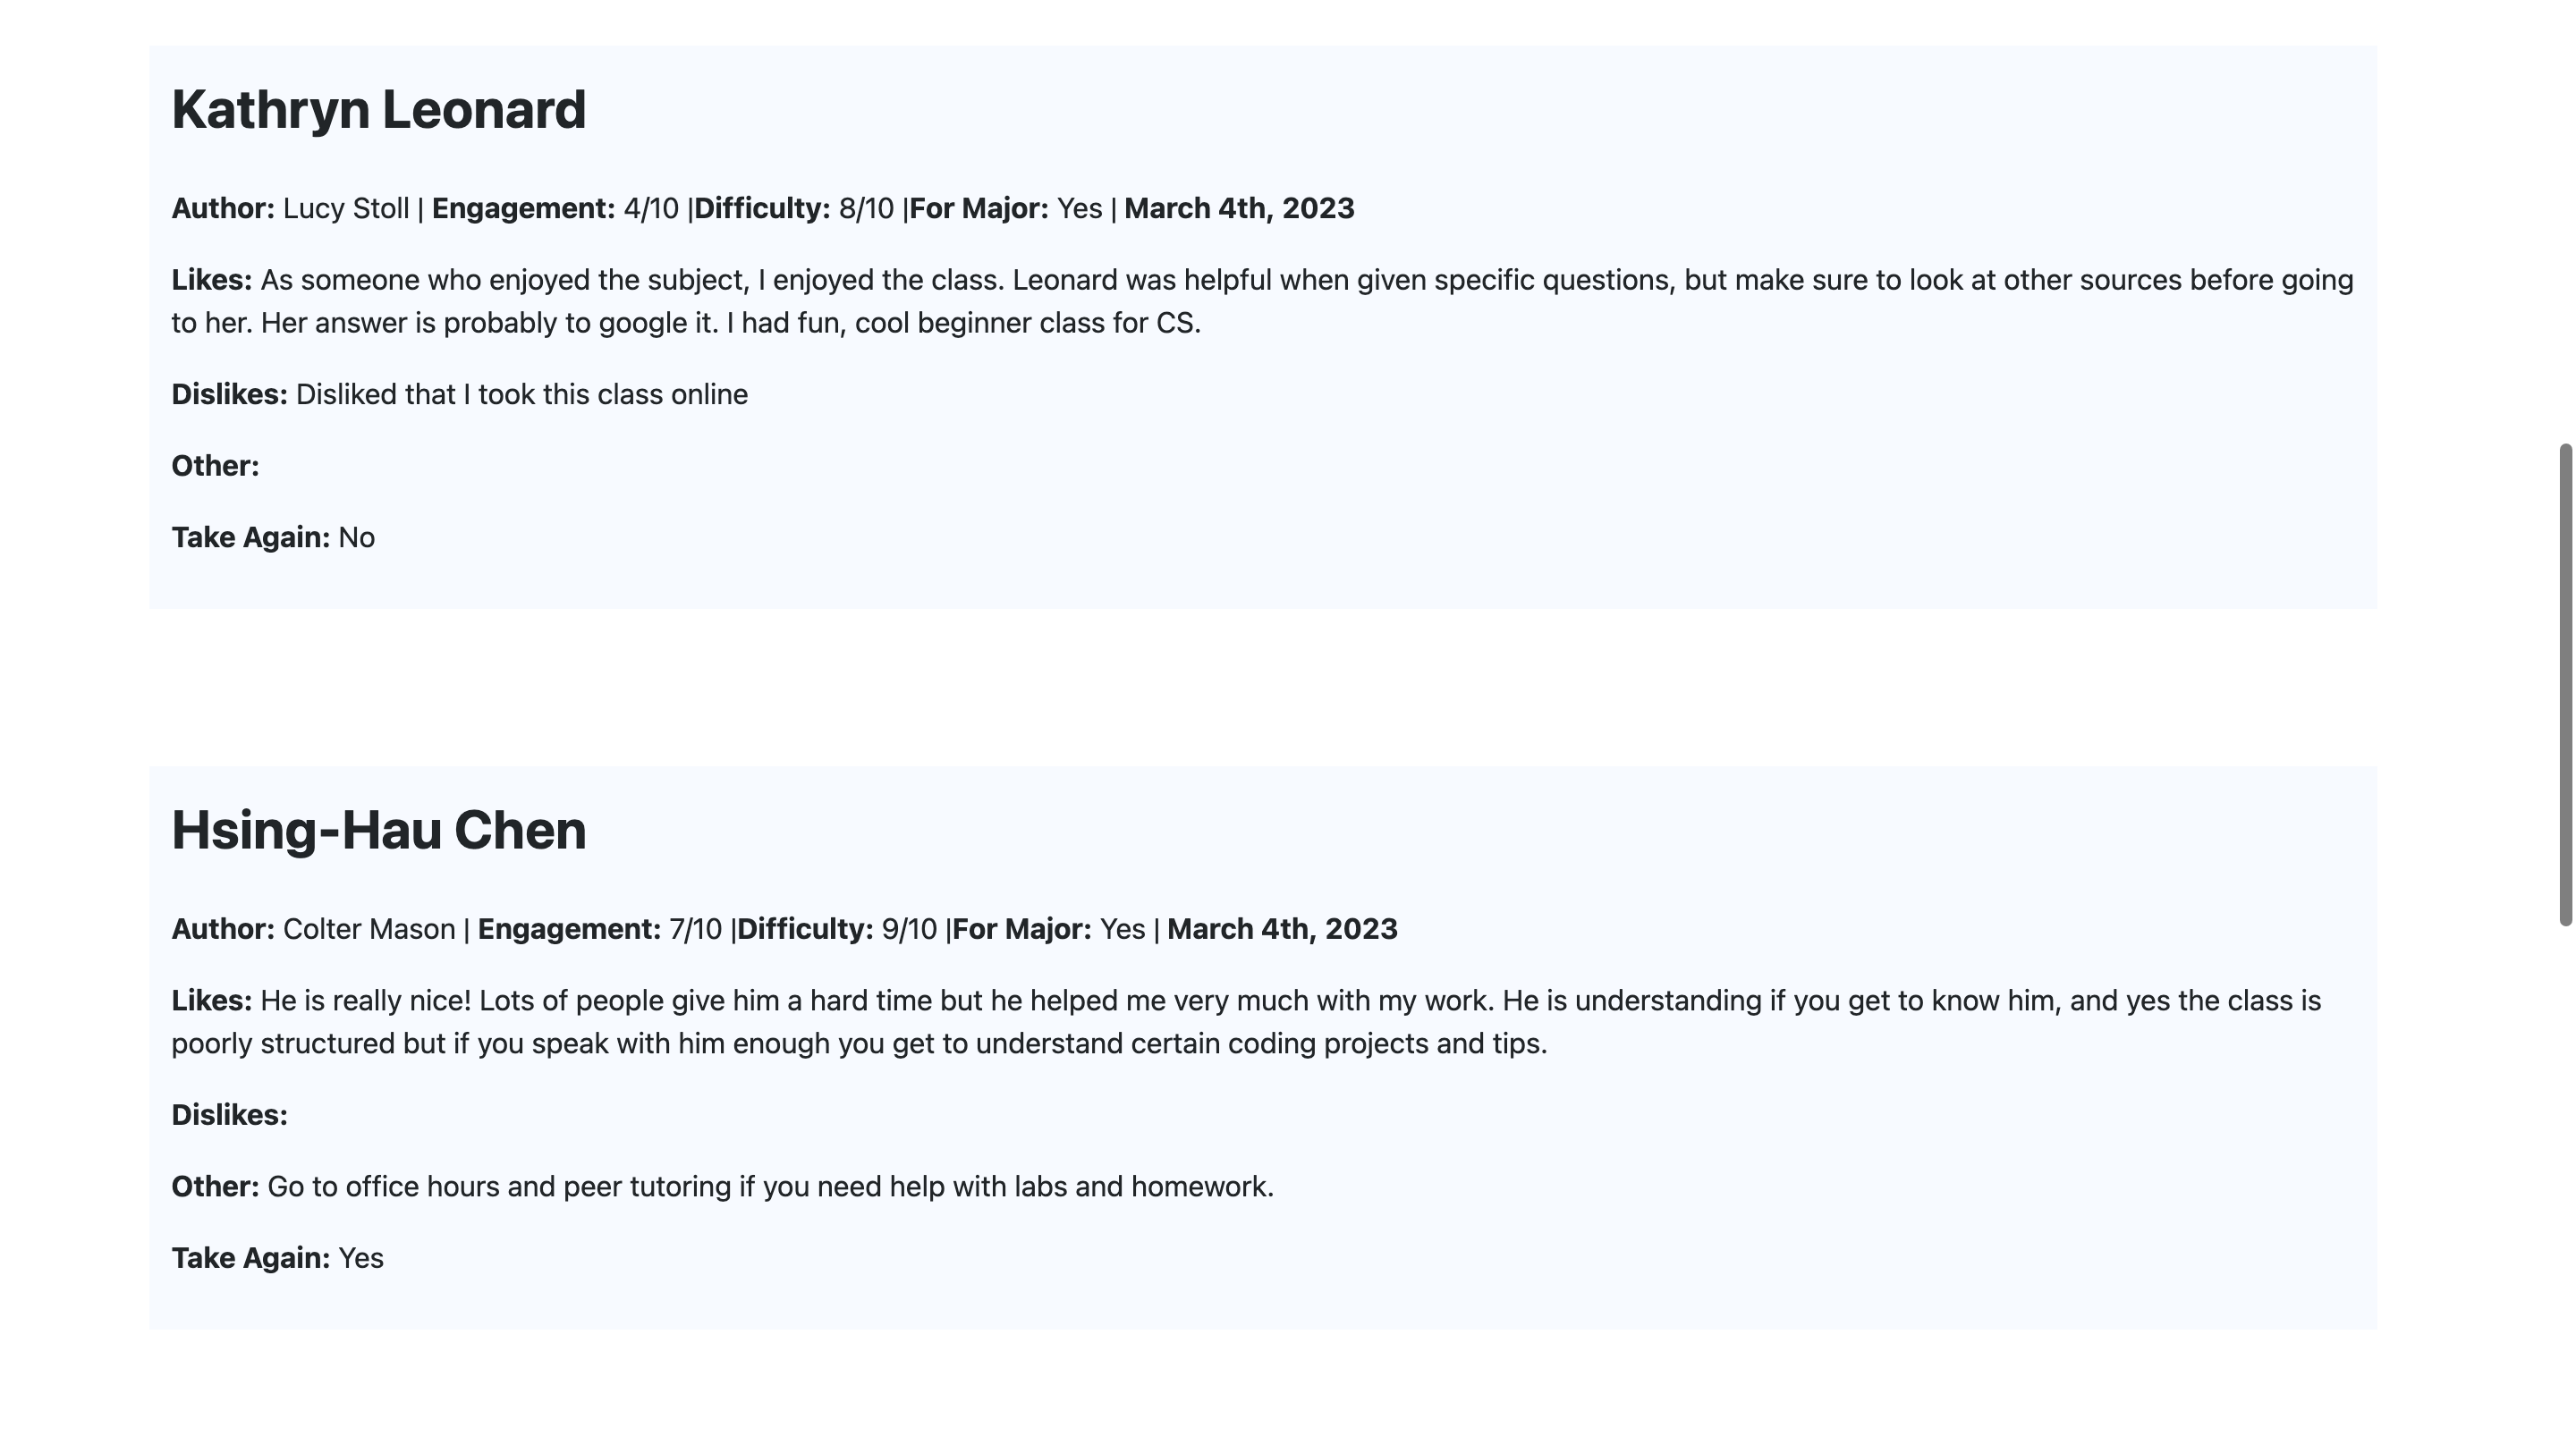
\includegraphics[scale=.175]{UT7}\\ \textbf{\footnotesize{Figures 6 and 7. Pie Charts with S}}\\

Ultimately I decided to stick with the pie charts as the only visual representation of data for my reviews. I made this decision because the pie charts were extremely difficult for me to implement within React, and I felt as though I did not have enough time to produce a well developed front-end app while also conducting more user testing with additional visual data and potentially being tasked with adding more visuals within my React app. In addition, the pie charts proved themselves to produce a lot of mixed feedback in the way they were presented which took many rounds of user testing to decide on a presentation of the pie charts in a way that communicated the necessary information effectively and efficiently. 

\subsubsection{Results and Discussion Regarding User Testing}

While numerous feedback and alternative ideas for user testing were available, this section focuses on highlighting the most significant concepts. Addressing every suggestion is impractical, and therefore, emphasis has been placed on the ideas I felt were most important for the enhancement and effectiveness of the user testing process. Overall, I recognize that it is essential to ensure that the chosen feedback adequately represent the range of feedback and ideas received during the testing process.

\subsection{Web App Development}
The web app development side of my project occurred concurrently with the user testing and involved many stages: 

\subsubsection{Design and Prototyping}
In the design and prototyping stage, I created mock-ups of the web app first using drawn sketches, and then using tools including google slides and canva. These mock-ups were used to get feedback from potential users and make any necessary changes before proceeding with development.

\subsubsection{Front-End Development}
In the front-end development stage, I used React to build the user interface for the web app. I used HTML, CSS, and TypeScript to create the various components of the app, such as the front page, search bar, pie charts, and course rating form.

\subsubsection{Conclusion}
In conclusion, my front-end development decisions for the web app were the result of careful consideration and strategic choices. I opted for React over Angular due to its simplicity, flexibility, and suitability for a modular design, aligning well with our emphasis on a dynamic user interface. The choice to use TypeScript was driven by its ease of understanding and the opportunity for continuous learning, as I already had existing familiarity with JavaScript.

In terms of libraries and frameworks, Infragistics emerged as the preferred solution for pie charts, offering robust capabilities and extensive customization options. Bootstrap was selected for styling, providing a responsive grid system, pre-designed components, and seamless integration for a visually consistent design across devices. Papaparse stood out for its efficiency in parsing CSV files, ensuring fast and reliable data processing, particularly beneficial for handling large datasets.

These choices were made with a focus on familiarity, ease of integration, and alignment with project-specific requirements. These technologies contribute to a efficient front-end development process, resulting in a user-friendly and visually compelling web app tailored for students in the Computer Science major at Occidental College.


\section{Evaluation Metrics}

%to do 
The success of the project was evaluated using mainly qualitative methods. The evaluation focuses on the usability and effectiveness of the platform in helping students make informed decisions about course selection.

\begin{enumerate}
\item User testing: In the end, I conducted a final round of user testing with participants to gather feedback on the platform's usability and effectiveness in helping them make informed decisions about course selection.\\


\item User interviews: I conducted interviews with a subset of my scope to gather more detailed feedback on their experience with the platform and how it could impact their course selection process.\\


Here were some of the interview questions:
\begin{itemize}
\item What unique aspects of this platform do you find most valuable compared to alternatives?
\item To what extent do you believe the web app has influenced or could influence your decision-making process when selecting courses or professors?
\item Did you find the platform easy to navigate? Why or why not?
\end{itemize}
\end{enumerate}

For my project, where the emphasis is on user interface design, ease of use, and supporting informed decision-making, qualitative methods provide a more comprehensive evaluation. While quantitative metrics like page views can offer some insights, qualitative methods ensure a deeper understanding of the user experience, helping to identify specific areas for improvement and refinement in the front-end design. In addition, I cannot use any quantitative metrics as my site is not yet fully functional, so data such as site engagement and reviews submitted do not exist. However, if I were to continue this project in the future, the data from my site could provide insight into the usefulness of my site. Overall, the combination of user testing and interviews allows for a holistic evaluation that goes beyond functionality to assess the platform's overall effectiveness in meeting the needs of its users.


\section{Results and Discussion}

\subsection{User Testing Results and Discussion}

The user testing phase provided crucial insights into the user experience and the effectiveness of the review platform. The initial hand-drawn reviews went through several iterations based on user feedback. Participants expressed the need for more visual elements in order to quickly scan an overview of the professors included in the reviews. Consequently, pie charts were introduced to visually represent the grading and teaching styles.

Despite improvements, challenges persisted in terms of clarity and repetition of pie charts, especially when multiple reviews were for the same professor. The transition from hand-drawn to digital reviews addressed some issues, allowing for greater flexibility and potential interactive elements. Participants appreciated the addition of a like/dislike button, providing a quick and intuitive way to express opinions on the review. However, the placement of these buttons within each section led to confusion, prompting a redesign to have a single set of buttons at the bottom of each review.

The incorporation of pie charts in the digital format remained a key element, but simplification was necessary due to technical challenges and user confusion. This demonstrated the importance of balancing visual appeal with simplicity and functionality.

\subsection{Web App Development Results and Discussion}

The development of the web app focused on translating insights gained from user testing into a functional and user-friendly platform. The key components included course and professor review sections, featuring pie charts to represent grading and teaching styles. Limiting pie charts to one set per professor addressed repetition issues. The like/dislike button was retained at the bottom of each review to encourage user engagement.

The choice to allow users to provide their names aimed to foster a positive environment \cite{ellis1984}. The iterative design approach was evident throughout the development process, refining visual elements and enhancing the user interface based on user testing insights.

\subsection{Results in the Context of Project Goals}

To assess the effectiveness of the web app in meeting project goals, I conducted final rounds of user testing and user interviews with the finished product. Participants engaged with the platform to evaluate its usefulness in the course selection process.

The user testing sessions were paired with a subsequent interview and revealed positive responses from participants, indicating that the platform was perceived as helpful in guiding course decisions. The incorporation of visual elements, such as the pie charts representing grading styles and teaching approaches, was particularly helpful for providing a quick and informative overview.

Participants expressed satisfaction with the user-friendly interface and the ability to access reviews encompassing both course and professor quality. The presentation of information contributed to a positive user experience, aligning with the project's aim to offer an effective and efficient platform for students to rate and review Oxy's CS courses.

While the positive reviews are helpful, it's crucial to acknowledge the potential presence of positive feedback bias. Participants may be inclined to provide positive feedback as a way to avoid confrontation or a desire to support the project creator. Recognizing this bias emphasizes the importance of ongoing user testing and feedback collection to iteratively refine the platform and combat potential biases.

Regarding future considerations, efforts can be made to address positive feedback bias by actively seeking critical input, conducting blind testing, or utilizing interviewers who are independent to the project. These strategies contribute to a more robust and unbiased evaluation of the platform's effectiveness in achieving its intended goals.


\subsection{Insights into Student Decision-Making}

The interview stage revealed a critical shift in project focus, emphasizing the importance of both classes and professors in shaping students' academic experiences. Participants in the interviews expressed a desire for a more holistic perspective, recognizing that the quality of education depends on both course content and the professor's teaching style and effectiveness. This insight prompted the adaptation of the project to accommodate a dual focus, aiming to provide a more comprehensive platform. This adjustment aligns the platform more closely with the needs of students within the Occidental Computer Science major, fostering a user-centered and well-rounded resource.
 
In addition, participants questioned the reliability of like/dislike metrics, emphasizing the need for careful implementation of user-generated features. Future iterations could explore alternative methods for gauging review helpfulness and credibility. There were also concerns about reviews from non-majors, which prompted considerations for major-specific perspectives. Future iterations could explore features allowing users to filter or prioritize reviews based on the reviewer's major, catering to diverse academic backgrounds.

\subsection{Future Research and Considerations}

The completion of this project marks a significant step towards creating a resource for the Occidental community. However, there are areas where future research can extend the insights gained from user testing.

In hindsight, I recognize that more user testing could have been accomplished throughout this process. As this was my first experience with user testing, I was new to the fast paced process of taking in the feedback, analyzing it, and quickly producing another new and improved mock-up. Another aspect of the project that hindered my ability to quickly produce mock-ups was in the later stages of user testing when it took me longer to create things on the front-end side than it was if I was a more experience front-end designer. I recognize that constant user testing is imperative for any web app to be successful and acknowledge that this process could be expedited if repeated in a future project.


\subsubsection{Incorporating Eye Tracking Technology}

Future research could benefit from the incorporation of eye-tracking technology during user testing sessions. This would provide a more nuanced understanding of users' visual attention and interaction patterns within the web app. By tracking eye movements, researchers, like myself, can gain insights into which elements attract users' attention, the sequence of their interactions, and potential areas of confusion or disinterest \cite{benway99}.

Eye-tracking technology could be particularly valuable when assessing the effectiveness of visual elements, such as pie charts. Understanding how users engage with and interpret these visual representations can inform further refinements to optimize user comprehension and satisfaction \cite{benway99}.



\section{Ethical Considerations}
The goal of this project is to develop a front-end website that can facilitate the course selection process for those involved with or interested in the Computer Science courses at Occidental College. While this system has the potential to greatly benefit both students and instructors, it also raises important ethical concerns related to data bias, transparency and explainability, and potential for abusive content. Therefore, this section aims to explore these issues and present strategies for mitigating them.

\subsection{Accessibility}
Accessibility and transparency are critical ethical concerns that must be addressed in the development and implementation of website for Oxy's CS course reviews \cite{shin2022}. The platform must be accessible to all students within the scope, assuming they have access to the internet, regardless of their abilities, to ensure equal opportunity to participate and provide feedback.

To address ethical concerns, the finished website prioritizes accessibility and transparency. Using React, I've ensured the site is user-friendly for everyone, including those with disabilities. I achieved this by incorporating accessibility-focused tools like React Accessibility and adhering to recognized web accessibility guidelines like WCAG 2.0 \cite{noname08}. The design keeps things simple, making navigation easy and complying with accessibility standards. The completed website features a consistent and intuitive design with a fixed menu bar across all pages, ensuring a straightforward and accessible user experience. Additionally, clear and concise page titles and descriptions contribute to a palatable and straight-forward explanation of where the user is within the site. This ongoing commitment to inclusivity reflects in the project's design even after its initial development. 

There is a considerable body of literature regarding ways to make websites as accessible as possible. In 2022, the ASIS\&T Standards Committee wrote a paper discussing why accessibility is so important in creating an information-resilient society \cite{dickey2022accessibility}. In this paper, they look at the "Digital Library Accessibility and Usability Guidelines that support blind and visually impaired users who rely on screen readers to interact with digital libraries", an important resource that I plan to use if I carry this project forward into next semester, but didn't focus on this semester due to time constraints \cite{dickey2022accessibility}.


I have also conducted user testing with accessibility in mind to identify any areas of confusion or difficulty in navigation, and make necessary adjustments based on feedback. Additionally, I provided clear instructions to help users understand how to use Course Companion effectively. Failure to address these accessibility and transparency concerns could result in excluding some students from the platform, as well as eroding trust and damaging the reputation of the college. By implementing these measures, I hope to ensure that the website is accessible and easy to use for all students.

Lastly, I chose Bootstrap for my web app mainly to make the site more accessible. Bootstrap is known for its user-friendly design components and adherence to accessibility standards. By using Bootstrap's built-in features like a responsive grid system, I aimed to ensure that the website is easy to navigate and provides a consistent experience for users on different devices. This decision reflects my commitment to creating a platform that is not only visually appealing but also accessible to a diverse audience.

It should be noted that there are many ways to enhance and improve the accessibility of my site, and future research could include more ways to make the site more accessible to all community members.

\subsection{Data Bias}
One of the ethical concerns that may arise from this project is data bias. The data used to generate ratings for classes may not accurately represent the experiences of all students. For example, some groups of students may be less likely to participate in rating their classes due to language barriers or because they are not comfortable sharing their opinions. This can result in a skewed representation of the student body's experiences with the classes offered. Additionally, ratings may be influenced by factors such as race, gender, or socio-economic status, which can lead to biased results \cite{dubrovina23}, \cite{chae17}. This section of my paper explores ways to avoid data bias in my project.

In terms of coding, it is often hard to avoid the presence of data bias in one's project. However, despite this, to address the issue of data bias, I have taken several steps. Firstly, I tried to access a wide range of individuals throught my user testing and user interviews. This including a good balance between genders, class years, and a balance between majors and non-majors. Accessing a diverse range of opinions helps to make sure I am getting well-rounded feedback in order to ensure my project isn't catered to a specific smaller group within the scope (i.e. only majors or only seniors)

Another important consideration to mitigate data bias is encouraging diverse user participation. Anonymity in the rating system can help reduce the impact of potential biases and encourage more honest feedback from students. In addition, it has been proven that anonymity within course evaluations provides a safer environment for students to share their most authentic feelings \cite{ellis1984}. By giving students the choice to submit their reviews anonymously, it might not only provide a more accurate representation of the courses, but it can also help to amplify the voices of underrepresented groups whose feedback may not have been previously heard. However, while I considered the benefit of having anonymous reviews, I ultimately decided to keep in the option to sign your review in order to promote accountability and avoid abusive content. While I decided to keep in the option to sign a review, users still retain the ability to submit a review anonymously. In addition, I will only use data that has been voluntarily submitted by students who have taken the courses. 

In terms of future considerations, having a back-end would require me to continuously monitor the data set for any potential bias and make adjustments as needed. However, one issue that may occur from this is my own personal bias. Because there would only be one person monitoring the data set, it could open the possibility of my personal beliefs being factored in to what should be deemed inappropriate/harmful/biased. One way to address my own bias when monitoring the data set is to send out a form to help identify what students' deem inappropriate and/or biased. This way, I can use the opinions of my peers to inform my decisions surrounding whether a review is biased. 

%\subsection{Privacy and Security}
%Privacy and security are also important considerations for the website. The platform collects and stores sensitive personal data from students, including their course ratings, recommendations, and feedback, which raises significant privacy concerns. Without security measures, this data could be at risk of unauthorized access or hacking attempts, potentially leading to identity theft or other malicious activity. Additionally, data breaches could reflect poorly on the Oxy community and lead to damage to the reputation of the college, which would have lasting effects.

%Celia Chen: Just use google auth or auth0 to do this for you (password protection). You just need to store the token those apis return you. Do not even attempt to create a user table where you store an email and a password since it is not the main focus of your project

% To mitigate these risks, I plan on implementing industry-standard security protocols. As I am using the Java Spring Boot framework for the back-end, I plan on taking advantage of its built-in security features, such as Spring Security, which provides session management and authorization out of the box. However, it is important to note that the security of the site will also depend on the security measures implemented by the Firebase database, which I will be using for data storage. Additionally, I plan on ensuring that only authorized personnel have access to the data, and that data is not shared with any third parties without students' consent. By prioritizing privacy and security, I hope to ensure that students' sensitive information is protected and treated with respect.

 % add abusive content section when finished withe the ethical paper template
\subsection{Abusive Content}
Abusive content is an important and relevant ethical concern that has affected many online platforms \cite{barker19} \cite{mishra19} \cite{keller18}. In terms of my project, my website allows students to rate and recommend their classes to their peers, which could lead to the posting of harmful or abusive comments about instructors or classmates. The potential for abusive content could also be exacerbated by the option of anonymity provided to users of the website\cite{ellis1984}. 

% cite a couple things that use guidelines to address appropriate conduct
In recent years, there has been a wide amount of research done on effective ways to detect and combat abusive content \cite{yadav15}\cite{fale22}\cite{yu16}. I  addressed this issue by drawing from the aforementioned sources, creating plans to implement clear guidelines for appropriate conduct on the website, and actively moderating user comments to prevent any abusive language or behavior. 

There are a few ways I plan to combat abusive content on my site. One of which is a reporting system. While I have not yet made a way for users to report reviews, user reporting is an important front-end solution for addressing abusive content on online platforms, and I recognize that it would be necessary to implement in further stages of my project. User reporting involves providing users with a straightforward and accessible system to report various forms of inappropriate behavior, such as harassment, hate speech, or the sharing of inappropriate content. This reporting system serves as a direct channel through which users can signal concerns, enabling the platform to take prompt and appropriate action in response to violations of community guidelines. 

Another way to address abusive content is to outline specific community guidelines. Eventually, In the footer of my site I plan on linking "site rules" which outline the types of reviews that would be inappropriate to have on the site. This includes reviews that contain inappropriate language and slander. In this set of rules I would give examples of reviews that are acceptable and reviews that are unacceptable. In addition, I would do user testing with this set of rules in order to incorporate feedback from the Occidental Community. Lastly, at the bottom of the review form, there is a checkbox that asks if the reviewer is sure the content of the review is appropriate for public consumption. 

\subsection{Conclusion}
In conclusion, while building a website that allows students to rate and recommend classes can be an incredibly useful tool, it is important to consider the potential ethical concerns that may arise from such a platform. Data bias, accessibility, and the potential for abusive content all need to be considered throughout the development and implementation of this project. By being mindful of these issues, it is possible to create a platform that is not only effective but also ethically responsible.

\appendix
\section{Replication Instructions}

To replicate the project, follow these instructions:\\


\textbf{Prerequisites:}
\begin{enumerate}
    \item Node.js (>=14.x)
    \item npm (Node Package Manager)
    \item Git\\
\end{enumerate}

\textbf{Step 1: Clone the Repository}\\


git clone https://github.com/kylaallen/SeniorComps.git

cd SeniorComps


\textbf{Step 2: Install Vite}\\


npm install -g create-vite\\


\textbf{Step 3: Create a New Vite Project}\\

create-vite my-project --template react-ts
cd my-project\\


if this creates an error, you may need to run this command 

first, then try again:\\


Set-ExecutionPolicy -Scope Process -ExecutionPolicy 

Default\\


\textbf{Step 4: Install Dependencies}\\

npm install\\


\textbf{Step 5: Install Additional Libraries}

\textbf{(You can do this in your IDE of choice or the terminal)}\\


npm install @infragistics/igniteui-react-core 

@infragistics/igniteui-react-charts\\


*note infragistics may require you to download on their 

site\\


npm install bootstrap\\


npm install papaparse\\

npm i react-router-dom\\


\textbf{Step 6: Start the Development Server}\\


npm run dev\\


This will start the development server, and you can view the web app by navigating to http://localhost:5173 in your browser.\\


Notes:
Ensure you have the required permissions and dependencies installed.
Package versions are omitted, so the latest versions will be installed.
These instructions aim to guide another CS student in replicating the project successfully.


\section{Software Architecture}
Course Companion is designed to be user-friendly. Users will be able to search for courses within the Computer Science major. Users will also be able to view and provide ratings and feedback on courses they have taken.\\


\centering 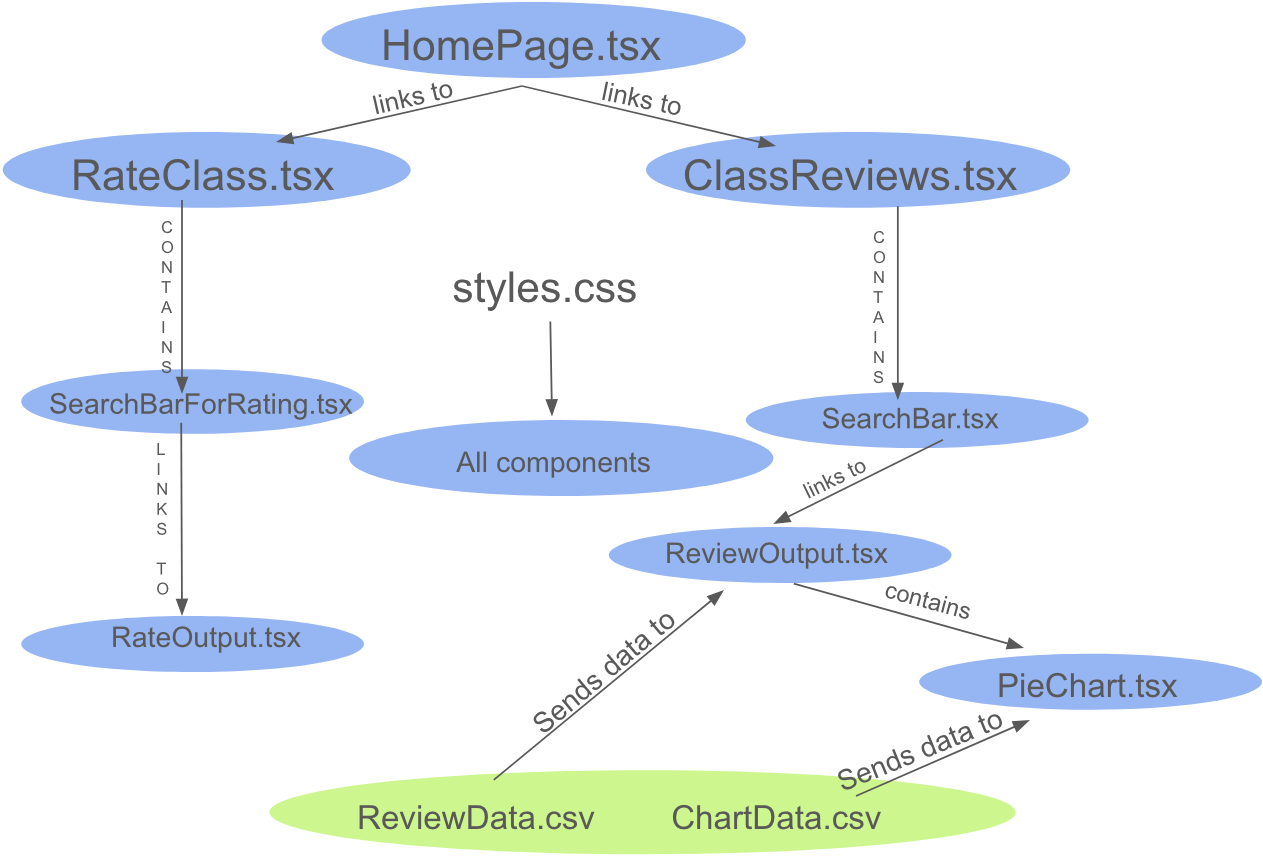
\includegraphics[scale=.4]{architecture}\\
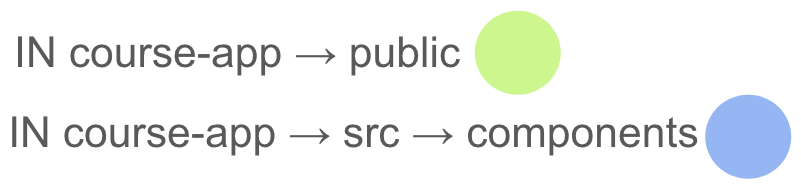
\includegraphics[scale=.35]{key}\\

Here are some key features of the user interface and their purpose:
\begin{itemize}
\item Home page: Displays a list of popularly rated courses, and a small blurb explaining the purpose of the site.
\item Search page: Allows users to search for courses based on various criteria and filter results by department, professor, and course rating.
\item Class Reviews page: Includes a search bar where users can search up and click on a class that they'd like to see reviews for.
\item Rate Class page:  Includes a search bar where users can search up and click on a class that they'd like to review.
\end{itemize}



\printbibliography

\end{document}
